% Created 2024-03-21 Thu 09:06
% Intended LaTeX compiler: pdflatex
\documentclass[11pt]{article}
\usepackage[utf8]{inputenc}
\usepackage[T1]{fontenc}
\usepackage{graphicx}
\usepackage{longtable}
\usepackage{wrapfig}
\usepackage{rotating}
\usepackage[normalem]{ulem}
\usepackage{amsmath}
\usepackage{amssymb}
\usepackage{capt-of}
\usepackage{hyperref}
\usepackage{placeins}
\usepackage{gensymb}
\author{Christian Johnson}
\date{\today}
\title{}
\hypersetup{
 pdfauthor={Christian Johnson},
 pdftitle={},
 pdfkeywords={},
 pdfsubject={},
 pdfcreator={Emacs 29.2 (Org mode 9.6.15)}, 
 pdflang={English}}
\begin{document}

\section{Screenshot}
\label{sec:orgcbcc9cd}
\begin{figure}[htbp]
\centering
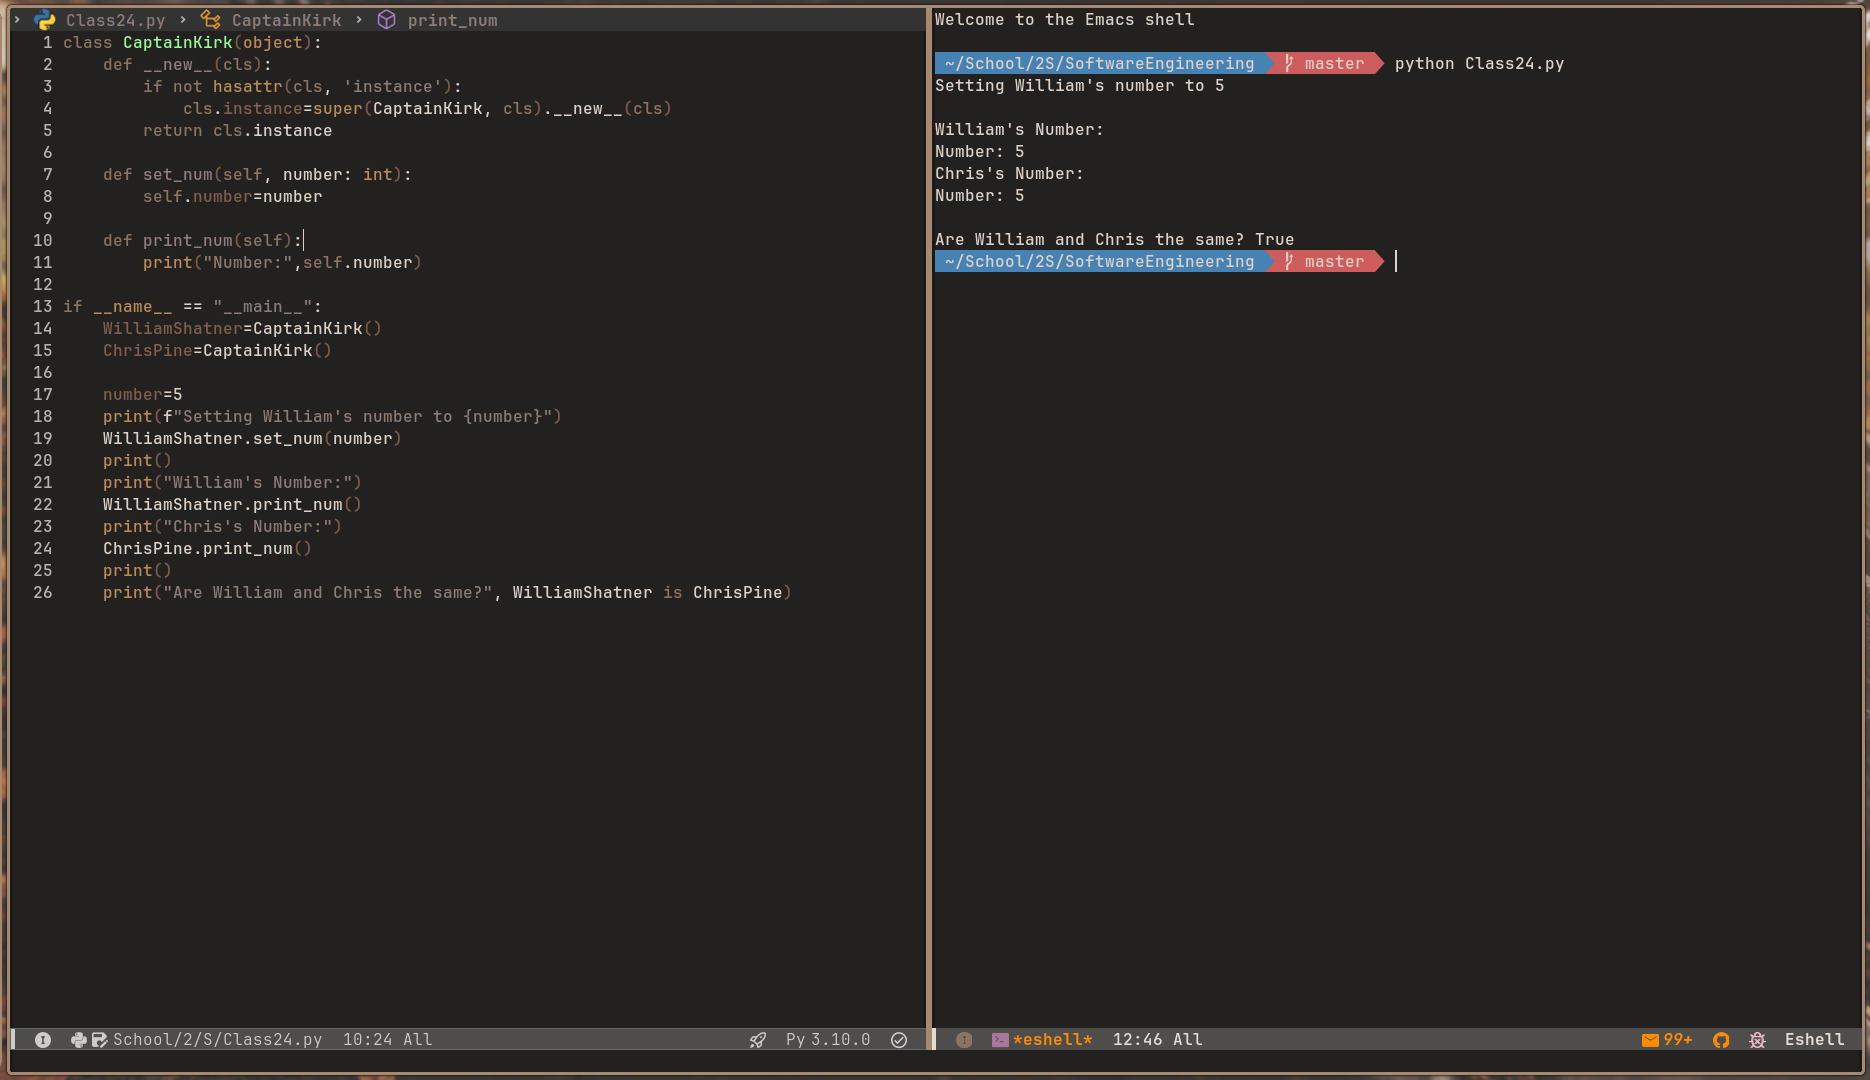
\includegraphics[width=.9\linewidth]{/home/csj7701/School/2S/SoftwareEngineering/Class24.png}
\bicaption{---}
\end{figure}

\section{Compile and run instructions}
\label{sec:org02b2bf6}

No compilation needed.
Simply navigate to the file's directory, and run the command \texttt{python Class24}.
If this does not work or throws an error, you may need to rename the file to \texttt{Class24.py}, then run the command \texttt{python Class24.py}, since D2L does not allow me to submit files with a \texttt{*.py} extension.
\end{document}
